\part{Exercice 23}

\begin{enumerate}
	\item[4.]
		\[
			\begin{cases}
				u_0 \in \R\\
				\forall n \in \N, u_{n+1} = u_n^2 + 1
			\end{cases}
		\]

		On pose \begin{align*}
			f: \R &\longrightarrow \R \\
			x &\longmapsto x^2 + 1
		\end{align*} et \begin{align*}
			g: \R &\longrightarrow \R \\
			x &\longmapsto x^2 + 1 - x
		\end{align*}

		\begin{center}
			\begin{tikzpicture}
				\tkzTabInit{$x$/1, $f$/2, $g(x)$/1}{$-\infty$, $0$, $+\infty$}
				\tkzTabVar{+/$+\infty$,-/$1$,+/ $+\infty$}
				\tkzTabLine{,,+,,}
			\end{tikzpicture}
		\end{center}

		\begin{center}
			\begin{tikzpicture}
				\tkzTabInit{$x$/1, $g$/2}{$-\infty$, $\frac{1}{2}$, $+\infty$}
				\tkzTabVar{+/{},-/$\frac{3}{4}$,+/{}}
			\end{tikzpicture}
		\end{center}
		
		$[0,+\infty[$ est stable par $f$, \[
			u_1 = f(u_0) \ge 1
		\] donc $u_1 \in [0, +\infty[$

		\begin{center}
			\begin{asy}
				import graph;
				size(0, 10cm);

				axes(EndArrow);
				
				real f(real x) {return x*x + 1;}

				draw(graph(f, -2, 3), magenta);
				draw((-1, 1)--(1, 1), red, Arrows);
				draw((-1,-1)--(f(3),f(3)));
				label("$y=x$", (f(3) + 0.5,f(3) - 0.5));

				real u0 = -1.3;

				label("$u_0$", (u0, -0.25), orange);
				label("$u_1$", (f(u0), -0.25), orange);
				label("$u_2$", (f(f(u0)), -0.25), orange);
				label("$\ldots$", (f(3) - 0.5, -0.25), orange);

				draw((u0,0)--(u0,f(u0)), dashed + orange);
				draw((f(u0),0)--(f(u0),f(f(u0))), dashed + orange);
				draw((f(f(u0)),0)--(f(f(u0)),f(f(u0))), dashed + orange);

				draw((u0, f(u0))--(f(u0),f(u0)), orange);
				draw((f(u0), f(u0))--(f(u0),f(f(u0))), orange);
				draw((f(u0), f(f(u0)))--(f(f(u0)),f(f(u0))), orange);
				draw((f(f(u0)), f(3))--(f(f(u0)),f(f(u0))), orange);
			\end{asy}
		\end{center}

		Donc, $\forall n \ge 1, u_n \in [0, +\infty[$.\\
		De plus, \[
			\forall n \ge 1, u_{n+1} - u_n = g(u_n) > 0
		\]
		Donc, $(u_n)$ croissante donc elle a une limite finie ou $+\infty$.\\

		On suppose que $u_n \tendsto{n \to +\infty} \ell \in \R$.\\
		Comme $f$ est continue, $f(\ell) = \ell$. Alors, $g(\ell) = 0$ : une contradiction

	\item[8.]
		\[
			u_0 \in [-2,2]\\
			\forall n \in \N, u_{n+1} = \sqrt{2 - u_n}
		\] 

		Soit $f: x \mapsto \sqrt{2 - x}$

		\begin{center}
			\begin{tikzpicture}
				\tkzTabInit{$x$ /1, $f$ /2, $g(x)$ /1}{$-2$, $1$, $2$}
				\tkzTabVar{+/$2$, R, -/$0$ }
				\tkzTabVal{1}{3}{0.5}{1}{1}
				\tkzTabLine{,+,z,-}
			\end{tikzpicture}
		\end{center}

		On pose $g: x \mapsto f(x) - x$ 

		\begin{center}
			\begin{tikzpicture}
				\tkzTabInit{$x$ /1, $g$ /2}{$-2$, $\alpha$, $2$ }
				\tkzTabVar{+/$4$, R/$0$, -/$-2$}
				\tkzTabVal{1}{3}{0.5}{$\alpha$}{0}
			\end{tikzpicture}
		\end{center}

		\begin{align*}
			g(\alpha) = 0 &\iff  \alpha = \sqrt{2 - \alpha} \\
										&\iff 
											\begin{cases}
												\alpha^2 = 2 - \alpha\\
												\alpha \ge 0
											\end{cases}\\
										&\iff \alpha = 1
		\end{align*}

		On pose \[
			\forall n \in \N, \begin{cases}
				v_n = u_{2n}\\
				w_n = u_{2n+1}
			\end{cases}	
		\]

		\[
			\forall n \in \N,
			\begin{cases}
				v_{n+1} = u_{2n+2} = f(f(u_{2n})) = f \circ f (v_n)\\
				w_{n+1} = u_{2n+3} = f\circ f (w_n)
			\end{cases}
		\] 

		\begin{center}
			\begin{tikzpicture}
				\tkzTabInit{$x$/1, $f\circ f$/2}{-2, 1, 2}
				\tkzTabVar{-/0, R/1, +/$\sqrt{2}$}
			\end{tikzpicture}
		\end{center}

		On pose $h: x \mapsto f(f(x)) - x = \sqrt{2 - \sqrt{2 - x}} - x$

		\begin{align*}
			\forall x \in ]-2,2[, h'(x) &= \frac{-\frac{-1}{2\sqrt{2-x}}}{2\sqrt{2 - \sqrt{2-x} } } - 1 \\
			&= \frac{1}{4\sqrt{2-x} \sqrt{2-\sqrt{2-x} } } -1 \\
			&= \frac{1-4\sqrt{4-2x - (2-x)\sqrt{2-x}}}{4\sqrt{2-x}\sqrt{2-\sqrt{2-x}}} \\
		\end{align*}

		$1 - 4\sqrt{4 - 2x - (2 -x)\sqrt{2-x}}$ a le même signe que \\$\left( 1 - 4\sqrt{4 - 2x - (2-x)\sqrt{2-x}} \right) \left( 1 + 4\sqrt{4 - 2x - (2-x)\sqrt{2-x}} \right)$ \\
		donc que $1 - 16\left( 4 - 2x - (2-x)\sqrt{2-x}  \right)$.\\

		On décide de passer par l'inégalité des accroissements finis.

		\begin{align*}
			\forall x \in ]-2,2[,
			\left| f'(x) \right| = \left| -\frac{1}{2\sqrt{2-x}} \right| = &\frac{1}{2\sqrt{2-x}} < 1\\
			&\iff \sqrt{2-x}> \frac{1}{2}\\
			&\iff 2-x > \frac{1}{4}\\
			&\iff x < \frac{7}{4}
		\end{align*}
		
		\begin{itemize}
			\item 
				Si $u_0 < \frac{7}{4}$ alors, \[
					\forall n \in \N, \left| u_{n+1} \right|  < M \left| u_n - 1 \right| 
				\] avec $M = \sup_{x \in ]-2, u_n[}\left| f'(x) \right| < 1$ \\
				Donc, $\left| u_n - 1 \right| < M^n \left| u_0 - 1 \right| \tendsto{n \to +\infty} 0$
			\item Si $u_0 > \frac{7}{4}$ alors $u_1< \frac{7}{4}\cdots$ (pas prouvé rigoureusement)
		\end{itemize}
\end{enumerate}
